\chapter{ที่มา ทฤษฎีและงานวิจัยที่เกี่ยวข้อง}
\section{บทนำ}

โดยทฤษฎีที่เกี่ยวข้องกับโปรเจคนี้มีหลากหลายสาขาด้วยกันโดยจะแบ่งเป็นส่วนของการเตรียมข้อมูลรูปภาพ โดยการใช้ Open source Computer Vision (OpenCV) เพื่อนำไปใช้กับส่วนของการทำ Optical Character Recognition (OCR), Tesseract OCR และส่วนของการทำ Natural language processing (NLP) โดยการใช้ Team Frequency Inverse Document Frequency (TF-IDF), Minimum Edit Distance,  Deep Cut ส่วนต่อไปคือสร้างระบบการค้นหาได้ใช้ Cosine Similarity และในส่วนการสร้างเว็บไซต์โดยใช้ RESTful API และส่วนสุดท้ายการทำ Word Embedding 

\section{แนวความคิดทางทฤษฎี}

\subsection{การเตรียมข้อมูลรูปภาพ}

เป็นการประมวลผลรูปภาพที่แปลงภาพให้เป็นข้อมูลทางดิจิทัลเพื่อใช้สำหรับปรับคุณภาพของภาพให้ตรงตามความต้องการ อย่างการตัดสิ่งรบกวน การลบกรอบ การหมุนรูป หรือการปรับให้ภาพมีความคมชัดมากยิ่งขึ้น ในโปรเจคของเรานั้นเอามาใช้ในการปรับคุณภาพของรูปภาพเพื่อช่วยให้การทำ OCR แม่นยำมากยิ่งขึ้น 

\subsubsection{คอนทัว (Contour) }

คอนทัว (Contour) \cite{doxygen} คือเส้นเค้าโครงของรูปภาพ ที่ไว้หาขอบเขตพื้นที่ที่มีค่าสีต่อเนื่องกัน หรือค่าเดียวกัน โดยใช้การเปลี่ยนให้รูปภาพอยู่ในรูปของ matrix และเช็คดูว่าค่าสีที่มีความแตกต่างอย่างชัดเจนเริ่มที่ตรงไหนและสร้างเป็นเส้นเค้าโครงขึ้นมาดังรูป \ref{fig:contour} ซึ่งการหาเส้นเค้าโครงจะทำงานได้ดีก็ต่อเมื่อเป็นรูปภาพแบบ Binary 

\begin{figure}[!h]
    \centering
    \includegraphics{contour}
    \caption{แสดงการหาเค้าโครงภายในรูป}\label{fig:contour}
\end{figure}

\subsubsection{การเปลี่ยนแปลงทางสัณฐานวิทยา (Morphology Transformation)}

เป็นกระบวนการเตรียมข้อมูลรูปภาพ  ที่จะทำการนำรูปภาพมาทำการเปลี่ยนแปลงลักษณะ รูปร่างของวัตถุภายในภาพ ปกติแล้วจะใช้ภาพที่เป็น Binary ซึ่งส่วนใหญ่จะใช้สำหรับการกำจัด 
noise การซ่อมแซมรูปร่างของภาพ หรือการเพิ่มขนาดให้กับวัตถุนั้นๆ โดยการทำการเปลี่ยนแปลงทางสัณฐานวิทยา (Morphology Transformation) นั้นจะมีวิธีการดำเนินการพื้นฐานอยู่ 2 วิธีคือการขยายภาพ และการกร่อนภาพ

Dilation คือการเพิ่มพื้นที่สีขาวของรูปเพิ่มพื้นที่สีไปตามขอบพื้นที่สีขาวและจะเปลี่ยนพื้นที่สีดำให้กลายเป็นสีขาวทำให้พื้นที่สีขาวมีความหนามากขึ้นดังรูป 

\begin{figure}[H]
    \centering
    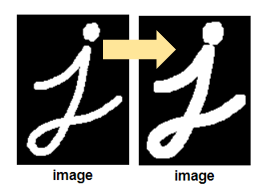
\includegraphics{dilation}
    \caption{แสดงการทำการขยายภาพ (Dilation) เพื่อเพิ่มพื้นที่สีขาว}\label{fig:Dilation}
\end{figure}

Erosion คือการกร่อนภาพ หรือก็คือจะลดพื้นที่สีขาวของภาพออกไปซึ่งวิธีการนี้ส่วนใหญ่จะใช้สำหรับการแยกสิ่งที่ของที่อยู่ติดกัน หรือลบ pepper noise ที่เป็น noise เล็กๆได้ โดยจะใช้หลักการเดียวกับการขยายภาพ  (Dilation) เพียงแต่จะเปลี่ยนจากพื้นที่สีขาวให้กลายเป็นพื้นที่สีดำดังรูป

\begin{figure}[H]
    \centering
    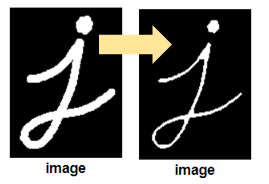
\includegraphics{erosion}
    \caption{แสดงการทำกร่อนภาพ (Erosion) เพื่อกร่อนพื้นที่สีขาว}\label{fig:Erosion}
\end{figure}

\subsection{Optical Character Recognition (OCR)}

OCR เป็นกระบวนการของการแปลงอักษรบนสื่อสิ่งพิมพ์ให้เป็นข้อความที่สามารถค้นหา เปลี่ยนแปลงและแก้ไขได้โดยที่ไม่ต้องพิมพ์ขึ้นมาใหม่ ด้วยการทำ Deep learning ในการเรียนรู้ภาพเพื่อแปลงออกมาเป็นตัวอักษร ซึ่งในโปรเจคของทางผู้จัดทำต้องทำระบบเกี่ยวกับค้นหาที่จะต้องคัดคำออกมาจากสิ่งพิมพ์เหล่านั้น จึงจำเป็นที่จะต้องใช้ OCR ในการแปลงภาพต้นแบบออกมาให้เป็นตัวอักษรก่อนที่จะนำไปใช้งานต่อ

จากการศึกษาพบว่าการทำ OCR ภาษาไทยนั้นมีอยู่มากมายในปัจจุบัน หนึ่งในนั้นมี T - OCR ซึ่งเป็น Library ของ AI For Thai \cite{nectec} และ Tesseract ของ Google \cite{google} ที่ใช้สำหรับแปลงภาพเป็นตัวอักษร โดยกลุ่มของเราเลือกที่จะใช้ Tesseract ในการทำ OCR เนื่องจากไม่เสียค่าใช้จ่ายเมื่อเทียบกับการใช้ OCR ของ AI For Thai นอกจากนั้นเรื่องของการเรียกใช้งานอย่างต่อเนื่อง Tesseract สามารถทำได้ดีกว่าเนื่องจากไม่จำเป็นต้องเรียกใช้งาน AI For Thai จากภายนอก

\subsection{Natural language processing}

Natural language processing คือกระบวนการที่ใช้ในทางปัญญาประดิษฐ์ซึ่ง เป็นกระบวนการที่ทำการวิเคราะห์ทางด้านภาษาซึ่งเอาไปประยุกต์ทำให้ปัญญาประดิษฐ์ (AI) สามารถทำให้คอมพิวเตอร์เข้าใจภาษาและตอบกลับได้ใกล้เคียงกับมนุษย์มากขึ้น โดยในโปรเจคนี้จะใช้มาช่วยในการหาคำสำคัญของหนังสือ และบทความต่าง ๆ เพื่อช่วยให้การค้นหาบทความมีประสิทธิภาพมากขึ้น

\subsubsection{Information retrieval}

Information retrieval คือ เทคโนโลยีการเก็บข้อมูลอย่างนึงโดยจะมีทั้งหมด 2 ลักษณะ ลักษณะที่ 1 คือ Boolean Retrieval เป็นการสร้างโครงสร้างข้อมูลในรูปแบบ Matrix ที่มีค่าเพียงแค่ 0,1 โดยที่ 0 คือไม่มีคำ (Term) ในหนังสือนั้น และ 1 คือมีคำ (Term) อยู่ภายในหนังสือนั้นหรือเรียกได้ว่าเป็น Term-Document Incidence  Matrix ดัง ตารางที่ 2.1 โดยที่ถ้าเราพิจารณาในรูปแบบแถวเราจะได้ Vector ของ Term นั้นที่ปรากฏอยู่ในหนังสือ ไหนบ้าง แต่การเก็บในรูปแบบ Boolean Retrieval เมื่อมีหนังสือ เยอะขึ้นจะทำให้เกิดค่า 0 ที่ไม่มีประโยชน์มากขึ้นจึงมีลักษณะที่ 2 คือโครงสร้างแบบ Inverted index เป็นการเก็บเพียง Term นั้นอยู่ภายในหนังสือ ไหนบ้างเพื่อจะเก็บแต่เพียงข้อมูลสำคัญเอาไว้ดัง ตารางที่ 2.2 โดย คำ (Term) จะผ่านกระบวนการเตรียมข้อมูลตัวอักษร ประกอบไปด้วย Tokenization (การตัดคำจากประโยชน์), Normalization (การจัดการคำย่อ), Stemming (การแปลงคำให้อยู่รูปแบบเดียวกัน), Stop words (จัดการคำที่ไม่มีความหมาย) เพื่อเป็นการจัดรูปของคำให้อยู่ในรูปแบบเดียวกันก่อนที่จะนำไปใช้งาน ซึ่งการเก็บข้อมูลแบบ Information retrieval (IR) จะทำให้การค้นหาข้อมูลภายในฐานข้อมูลได้อย่างรวดเร็วและมีประสิทธิ์ภาพ
\begin{table}[H]
\caption{Information retrieval ในลักษณะ Boolean Retrieval}\label{tbl:ir}
    \begin{tabular}{|l|c|c|c|c|c|}
        \hline
                  & Antony \& Cleopatra & Julius Ceasar & The Tempest & Hamlet & Othello \\ \hline
        Antony    & 1                   & 1             & 0           & 0      & 0       \\ \hline
        Brutus    & 1                   & 1             & 0           & 1      & 0       \\ \hline
        Ceasar    & 1                   & 1             & 0           & 1      & 1       \\ \hline
        Calpurnia & 0                   & 0             & 1           & 0      & 0       \\ \hline
        Cleopatra & 1                   & 0             & 1           & 1      & 1       \\ \hline
        Mercy     & 1                   & 0             & 1           & 1      & 1       \\ \hline
        \end{tabular}
\end{table}

    \begin{figure}[H]
        \centering
        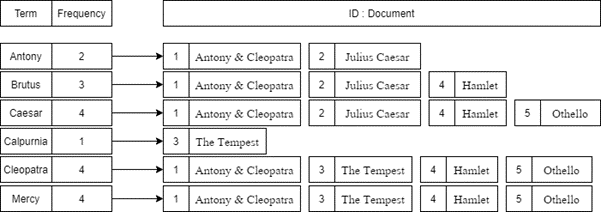
\includegraphics{ir}
        \caption{Information retrieval ในลักษณะ Index Retrieval}\label{fig:ir}
    \end{figure}

\subsubsection{TF-IDF}

เป็นเทคนิคในการคัดแยกคำตามความสำคัญผ่านการให้น้ำหนักในแต่ละคำ โดยแบ่งเป็นสองส่วนนั้นก็คือ TF (Team Frequency) เป็นการดูว่าคำนี้ หรือว่า Term นี้ปรากฏขึ้นภายใน document มากน้อยเพียงไหน และ IDF (Inverse  Document Frequency) คือการหาความผกผันในความถี่ของหนังสือโดยคะแนนความผกผันที่ทำให้รู้ว่าคำนี้เป็นคำที่มีความสำคัญเฉพาะภายในหนังสือนี้ แต่เนื่องจากการดูคะแนน IDF เพียงอย่างเดียวไม่สามารถบอกได้ว่า Term นั้นเป็นคำสำคัญ จึงจำเป็นต้องนำค่า TF มาคูณกับ IDF เป็นค่า TF-IDF เพื่อดูความสำคัญของ Term นั้น ในส่วนการคำนวณนี้เพื่อนำไปใช้ในการค้นหาแบบ Cosine Similarity ต่อไป โดยที่ TF จะใช้เป็น Log normalization โดยคำนวณได้จากสมการ 2.1 ซึ่ง $f_{t,d}$ คือความถี่ของคำ (Term) ที่ปรากฏขึ้นภายใน Document ส่วน IDF จะคำนวณจากสมการ 2.2 ซึ่ง N คือจำนวน Document ที่มีภายในระบบ และ $n_{t}$ คือ จำนวนของ document ที่มีคำ (term) นี้อยู่ เมื่อหาค่าทั้ง TF และ IDF ได้แล้วก็จะหาค่าของ TF-IDF ได้จากสมการ 2.3

\begin{equation}
    tf=\log{(1+f_{t,d})}
    \end{equation}

\begin{equation}
    idf=\log{\frac{N}{n_{t}}}
\end{equation}

\begin{equation}
    TF-IDF=tf*idf
    \end{equation}    

\subsubsection{Cosine Similarity}

เป็นหน่วยวัดความคล้ายคลึงกันระหว่างข้อมูลสอง Vector โดยวัดจากมุม cosine ของจาก Vector ทั้งสองโดยคำนวณได้จากสมการ 2.4 โดยที่ ||x||,||y|| คือ สมการของ Euclidean norm ของ Vertor x, y ดังสมการ 2.5 โดยในโปรเจคนี้เราได้นำค่าน้ำหนักของ TF-IDF มาเป็นน้ำหนักในการคิดค่า Cosine Similarity โดยนำประโยคที่จะค้นหามาผ่านกระบวนการเตรียมข้อมูลตัวอักษร ก่อนที่จะนำมาค้นหาว่า document ไหนมีค่า relevance score (คะแนนความสัมพันธ์) เพื่อนำมาเรียงค่าคะแนนสูงสุดแสดงเป็นผลลัพธ์การค้นหา


\begin{equation}
    \sin(x,y)=\frac{x*y}{\|x\|\|y\|}
\end{equation}    

\begin{equation}
    \|x\|=\sqrt{x_{1}^2+x_{2}^2+\cdots+x_{n}^2}
\end{equation}    
\subsubsection{Minimum Edit Distance}

เป็นหลักการที่หาระยะห่างที่สั้นที่สุดจากคำนึงไปสู่อีกคำนึงจะมีความแตกต่างกันเท่าไหร่ซึ่งจะหลักการเช็คความห่างของคำทั้งหมดสามรูปแบบ
\begin{itemize}
    \item รูปแบบ Insert(I) จะเป็นการเพิ่มตัวอักษรลงไปในคำนั้น เพื่อคำดั้งเดิมของเราจะเปลี่ยนแปลงเป็นคำที่เราต้องการ
    \item รูปแบบ Delete(D) จะเป็นการลบตัวอักษรออกไปในคำนั้น เพื่อคำดั้งเดิมของเราจะเปลี่ยนแปลงเป็นคำที่เราต้องการ
    \item รูปแบบ Replace(R) จะเป็นการเปลี่ยนตัวอักษรนั้นให้เป็นตัวอักษรใหม่ เพื่อคำดั้งเดิมของเราจะเปลี่ยนแปลงเป็นคำที่เราต้องการ
\end{itemize}
\begin{figure}[H]
    \centering
    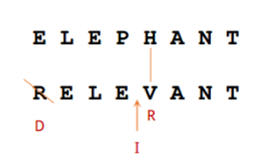
\includegraphics{editdistance}
    \caption{หลักการการเช็ค edit distance \cite{ritambhara}}\label{fig:editdistance}
\end{figure}
หลังจากมีรูปแบบการวัดระยะห่างของคำดังรูปภาพที่ \ref{fig:editdistance} แล้ว จะต้องทำการหาคำที่สั้นที่สุดผ่านรูปแบบของตารางดังรูปภาพที่ \ref{fig:minimumtable} ซึ่งการคำนวณผ่านตารางจะเป็นการนำการกระทำก่อนหน้ามาคำนวนเรื่อย ๆ จนได้รูปการเปลี่ยนเป็นคำใหม่ที่ใช้การเปลี่ยนน้อยที่สุด
\begin{figure}[H]
    \centering
    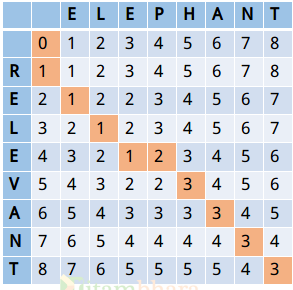
\includegraphics{minimumtable}
    \caption{ตัวอย่างตารางการทำ Minimum edit distance \cite{ritambhara}}\label{fig:minimumtable}
\end{figure}

ซึ่งในโปรเจคของเราได้ดึงหลักการ Minimum edit distance มาใช้ในการตรวจสอบหาคำที่สะกดไม่ถูกต้องโดยมีเกณฑ์ตั้งไว้ว่าถ้าเกินที่กำหนดไว้จะถือว่าคำ ๆ นั้นสะกดไม่ถูกต้องแล้วถูกแก้ให้เป็นคำที่สะกดถูกต้อง

\subsubsection{Spelling Corrector by Peter Norvig}

หลักการการแก้คำผิดของ Peter Norvig\cite{norvig} เป็นการนำคำที่ถูกพิมพ์เข้ามาสร้างมาเป็นคำใหม่โดยการแบ่งคำ การลบคำ การกลับคำ การแทนที่คำ การเพิ่มคำ 
และนำคำที่สร้างใหม่ไปเช็คในพจนานุกรมภาษาว่ามีคำที่สร้างใหม่คำนั้นหรือไม่ ถ้ามีให้นำคำที่ได้ไปหาค่าความน่าจะเป็นของคำที่มีโอกาสเกิดขึ้นมากที่สุด ซึ่งใน Library 
นี้ Norvig ได้นำไปหาโดยใช้ข้อมูลจาก Corpus ที่สร้างขึ้นจากคำที่ได้จาก Project Gutenberg\cite{guten}, Wikitionary\cite{wikitionary} และ British 
National Corpus\cite{kilgarriff} ที่จะรวมคำต่างเอาไว้ จากนั้นคำนวนความน่าจะเป็นของคำที่เกิดขึ้นโดยใส่คำที่ต้องการหาแล้วนับว่าใน Corpus นั้นมีคำนั้นปรากฏขึ้นเท่าไร
หารด้วยจำนวนคำของ Corpus ทั้งหมด ก็จะได้ความน่าจะเป็นออกมา ซึ่งคำที่จะแก้ก็จะเลือกจากคำที่มีค่าความน่าจะเป็นมากที่สุด โดย library PyThaiNLP\cite{pythainlp} และ Pyspellchecker\cite{pypi} 
นั้นก็ใช้หลักการเดียวกันกับการแก้คำผิดของ Peter Norvig 

\subsection{RESTful Service}
เป็นการสร้าง web service โดยเรียกใช้ผ่านทาง HTTP Method ทั้ง 4 ประเภท GET/POST/PUT/DELETE ส่งข้อมูลออกมาเป็นรูปของ XML ทำให้ปริมาณข้อมูลที่ส่งมาน้อยกว่าการใช้ Protocol SOAP  โดยโครงสร้างของ 
HTTP Request ดังรูปภาพที่ \ref{fig:httpreq} ประกอบด้วย 

\begin{enumerate}
 \item VERB: แสดง method ของ HTTP
 \item URI: ตำแหน่งของข้อมูลที่ต้องการ
 \item HTTP Version: เวอร์ชั่นของ HTTP
 \item Request Header: Metadata ที่เก็บข้อมูลในรูปแบบ Key-Value ของ header
 \item Request Body: ส่วนเก็บข้อมูลของเนื้อหา
\end{enumerate}

\begin{figure}[H]
    \centering
    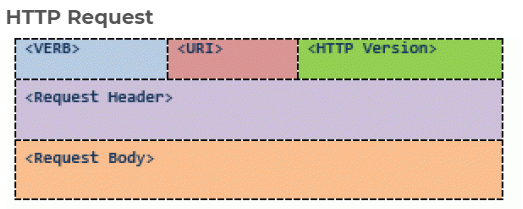
\includegraphics{httpreq}
    \caption{แสดงถึงโครงสร้างของ HTTP Request \cite{Saixiii}}\label{fig:httpreq}
\end{figure}

HTTP Response ดังรูปภาพที่ \ref{fig:httpres} ประกอบด้วย


\begin{enumerate}
	\item HTTP Version: เวอร์ชั่นของ HTTP
	\item Response Code: รหัสผลลัพธ์ของการทำงานในระดับ HTTP เป็นเลข 3 หลัก
	\item Response Header: Metadata ที่เก็บข้อมูลในรูปแบบ Key-Value ของ header
	\item Response Body: ส่วนเก็บข้อมูลของเนื้อหา

   \end{enumerate}
   
\begin{figure}[H]
    \centering
    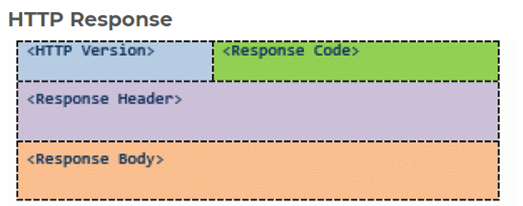
\includegraphics{httpres}
    \caption{แสดงถึงโครงสร้างของ HTTP Response \cite{Saixiii}}\label{fig:httpres}
\end{figure}

\subsection{Word Embedding}

เป็นวิธีการที่จะเปลี่ยนคำปกติเป็น vector ให้อยู่ในหลากหลายมิติเพื่อให้สามารถเปรียบเทียบคำต่าง ๆ (ซึ่งคำก็จะเป็นเสมือนจุดบนกราฟดังภาพที่ \ref{fig:embedgraph}) 
ว่ามีความสัมพันธ์ใกล้เคียงกับคำไหนบ้างในระบบโดยมาจากการ dot กันระหว่างเวกเตอร์ของคำ 
ซึ่งมิติใน word embedding นั้นจะเป็นการแสดงถึงการจำแนกประเภทของคำเหล่านี้ โดยที่เราจะสามารถกำหนดตัวเลขขึ้นมาและโมเดลจะทำการสร้างมิติ  
 โดยมีการทำ word embedding มากมายไม่ว่าจะเป็น Word2Vec \cite{xin} \cite{Goldberg} ที่ถูกสร้างโดยทีมวิจัยของ 
Google FastText \cite{fasttext} เป็น word embedding อีกหนึ่งตัวที่สร้างขึ้นจากทีมวิจัยของ facebook หรือจะเป็น ELMo \cite{matthew} 
ที่เป็นรูปแบบการ word embedding ที่ดูรูปคำโดยรอบเป็นต้น 

\begin{figure}[H]
    \centering
    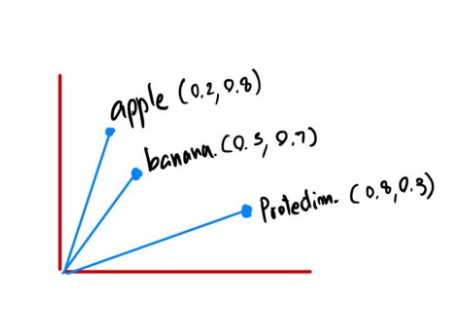
\includegraphics[scale=0.5]{embedgraph}
    \caption{ภาพแสดงการหาความสัมพันธ์ระหว่างคำโดยใช้วิธีการทาง word embedded \cite{lukkid}}\label{fig:embedgraph}
\end{figure}

จากภาพที่ \ref{fig:7Dto2D} จะแสดงให้เห็นว่าแต่ละคำใกล้เคียงกับอะไรบ้าง อย่างเช่น cat และ kitten
จะมีค่าในแต่ละมิติที่ใกล้เคียงกัน (ดูจากภาพมิติก็คือ living being, feline, human เป็นต้น ซึ่งจะถูกเรียนรู้ขึ้นมาโดยโมเดล ในที่นี้กำหนด ไว้ 7 มิติ)

\begin{figure}[H]
    \centering
    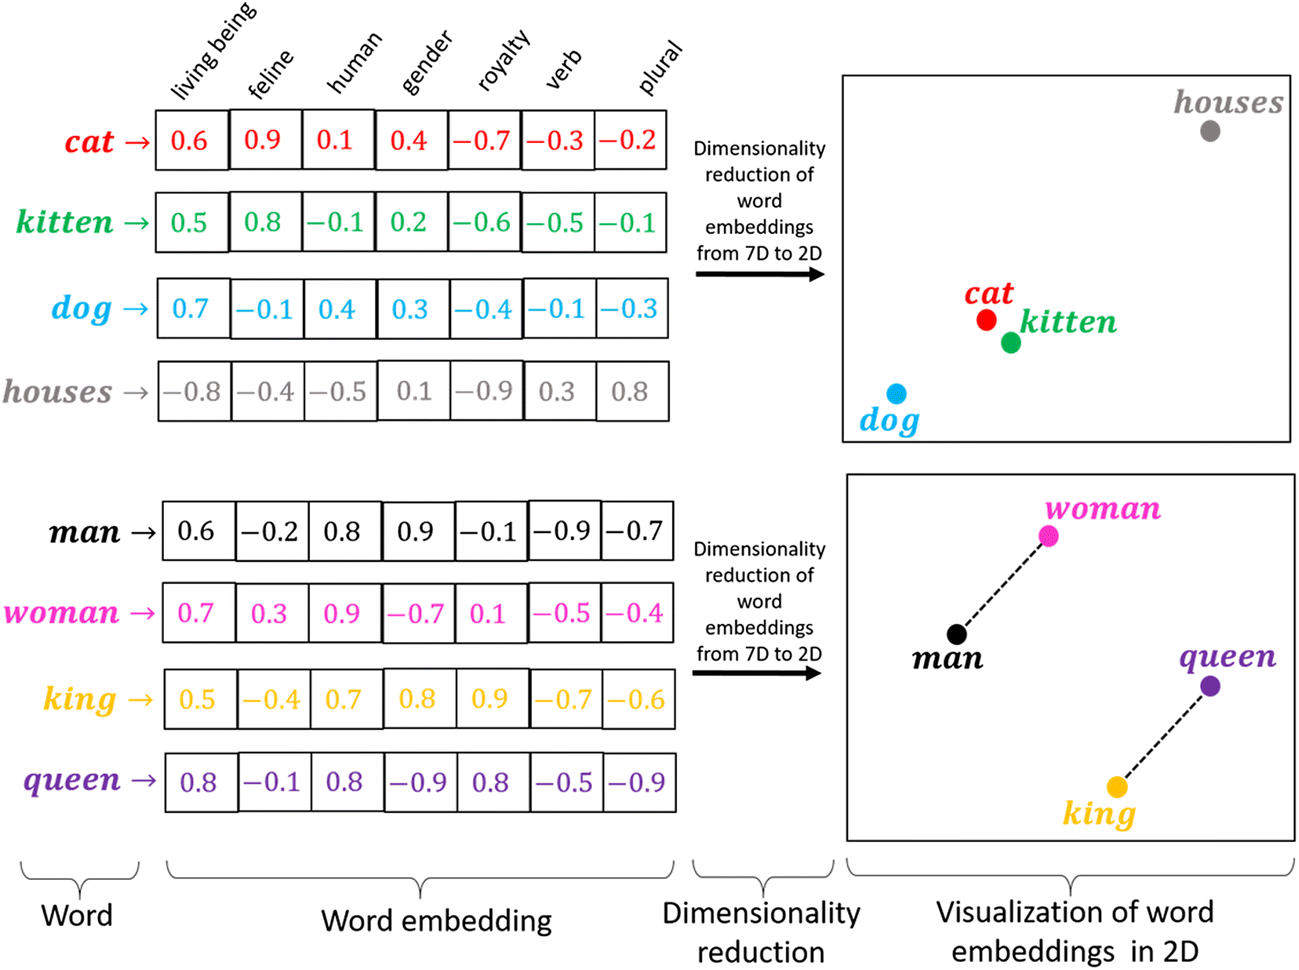
\includegraphics[scale=0.2]{7Dto2D}
    \caption{ภาพแสดงการหาความสัมพันธ์ระหว่างคำโดยใช้วิธีการทาง word embedded \cite{sasiwut}}\label{fig:7Dto2D}
\end{figure}


\subsubsection{Word2Vec}
ทฤษฎี Word2Vec\cite{shortStoryForWord2Vec} เป็นทฤษฎีที่ช่วยจัดการกับคำศัพท์ที่มีความหมายใกล้เคียงกัน หรือคำศัพท์ที่มีความสัมพันธ์อย่างคำตรงข้ามกัน 
อย่างคำว่า พระราชา กับ กษัตริย์ ที่เป็นคำที่ความหมายใกล้เคียงกัน แต่ตรงข้ามกับคำว่า ราชินี โดยทั้งหมดนี้จะถูกจัดเก็บในรูปแบบของเวกเตอร์
แน่นอนว่าการที่จะรู้ว่าแต่ละคำมีความสัมพันธ์ได้นั้น เราจำเป็นต้องสร้างประเภทของคำจากรูปประโยคอย่างเช่น “การ เลี้ยง หมา เป็น สัตว์เลี้ยง ถือ เป็น การ ผ่อนคลาย” 
กับ “แมว ถือ เป็น สัตว์เลี้ยง ที่ สุขุม” จากทั้งสองประโยคจะเห็นว่าคำที่เหมือนกันจากทั้งสองประโยค จะเป็นคำว่า สัตว์เลี้ยง ซึ่งการทำ Word2Vec 
จะเป็นการดึงประเภทโดยเช็คจากคำใกล้เคียงเพื่อจัดกลุ่ม ดังนั้นจากคำว่า สัตว์เลี้ยง ที่มีคำว่า หมา และ แมว เป็นสัตว์เลี้ยงเช่นเดียวกัน จะแสดงว่าคำว่า 
หมา และ แมว มีความหมายใกล้เคียงกันจากความสัมพันธ์กัน ทั้งนี้การที่แต่ละคำจะมีสัมพันธ์ที่เชื่อมโยงกันได้มาก หรือน้อยขึ้นอยู่ระยะของคำ (Window Size) 
ยกตัวอย่างถ้ามีค่ามาก คำว่าสัตว์เลี้ยงอาจจะมีคำที่ไม่เกี่ยวข้องเกิดขึ้นหากข้อมูลไม่เพียงพอ เช่น ตู้เย็น หมา แมว เป็นสัตว์เลี้ยง แต่ถ้าหากค่าน้อยเกินไป หมา 
อาจจะไม่ถูกนับเป็นประเภทสัตว์เลี้ยงแทน
นอกจากส่วนการใช้คำข้างเคียงมาช่วยในการทำ Word2Vec แล้วยังมีส่วนของรูปแบบการสร้างโมเดลเพื่อหาคำที่มีความสัมพันธ์กันอีกด้วย 
โดยจะมีสองรูปแบบคือ CBOW (continuous bag of words) จะเป็นรูปแบบของการที่ใช้คำหลาย ๆ คำเผื่อมาหาคำเพียงคำเดียว 
และ Skip-Gram ที่จะตรงข้ามกับรูปแบบที่แล้วคือ การที่ใช้คำหนึ่งคำเพื่อหาคำหลายคำออกมา

\begin{figure}[H]
    \centering
    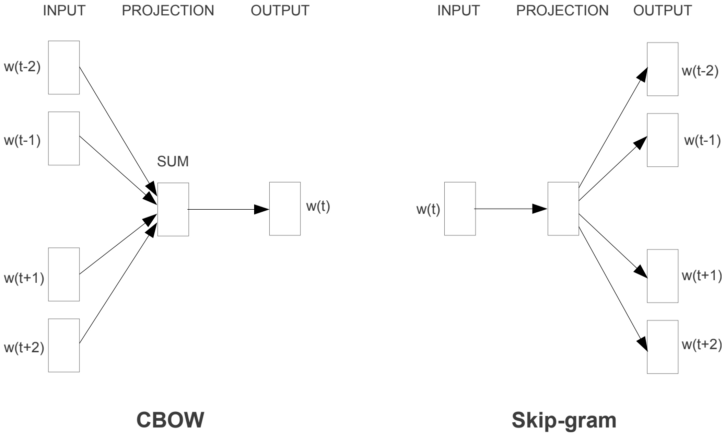
\includegraphics[scale=0.5]{cbowskip}
    \caption{ภาพแสดงโมเดล Skip-gram และ CBOW \cite{ichi}}\label{fig:cbowskip}
\end{figure}

\subsubsection{Skip-gram}

Skip-gram\cite{ichi} เป็นโมเดลที่จะใช้หาความสัมพันธ์ของคำ โดยจะนำคำที่เข้าไปไปหาคำบริบทโดยรอบ โดยการที่โมเดลจะทำการอ่านประโยคเข้าไปและเรียนรู้จากประโยค 
โดยการพิจารณาบริบทโดยรอบของคำ อย่างเช่น Thou shalt not make a machine in the likeness of human a mind โมเดลก็จะทำการรับคำ 
1 คำเข้าไปและพิจารณาคำรอบๆ เริ่มจากว่า not ก็จะพิจารณาสองคำก่อนหน้าและสองคำหลัง (ตามจำนวน window size ในที่นี้กำหนด window size เป็น 2) 
ซึ่งจะได้มา 4 คำ คือ Thou, shalt, make และ a ดังรูปที่ \ref{fig:skipgram} ซึ่งโมเดลก็จะทำการเรียนรู้คำไปเรื่อยๆเพื่อ weight น้ำหนักภายในโมเดล
\begin{figure}[H]
    \centering
    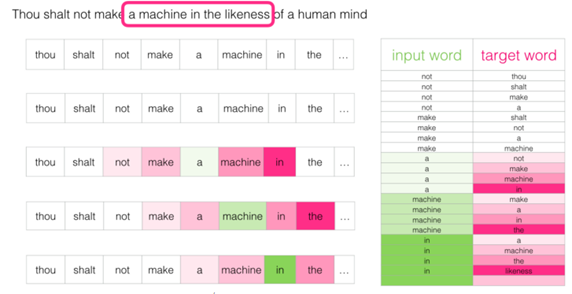
\includegraphics{skipgram}
    \caption{แสดงการทำงานของ Skip-gram \cite{ichi}}\label{fig:skipgram}
\end{figure}

\subsubsection{CBOW}
CBOW\cite{ichi} เป็นโมเดลที่จะใช้หาความสัมพันธ์ของคำแบบจะพิจารณาคำหลายๆคำเพื่อหาคำหนึ่งคำ ดังตัวอย่างในรูปที่ \ref{fig:cbow} โดยการที่โมเดล
จะทำการอ่านประโยคเข้าไปและเรียนรู้จากประโยคเหมือนโมเดล Skip-gram อย่างเช่น Thou shalt not make a machine in the likeness of human a mind 
โมเดลก็จะทำการอ่านคำตามจำนวน window size ถ้า window size เป็น 2 ก็จะเป็นการกำหนดว่าอ่าน input เข้าไป 2 คำและคำถัดจาก 2 คำนั้นในประโยคจะเป็น
ผลลัพธ์ที่ได้จาก input  อย่างเช่นถ้าใส่ thou,shalt เข้าไปก็จะได้คำว่า not ออกมา ซึ่งจะสร้างโมเดลนี้ก็จะต้องใส่ข้อมูลประโยคจำนวนมากเพื่อทำการ weight 
ค่าน้ำหนักภายในโมเดล ให้มีประสิทธิภาพคล้ายกับโมเดล skip-gram

\begin{figure}[H]
    \centering
    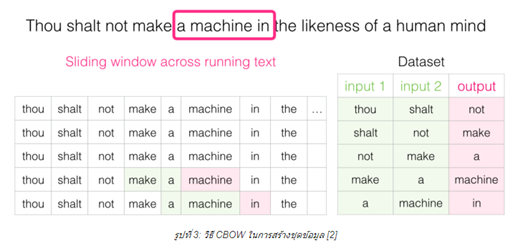
\includegraphics{cbow}
    \caption{แสดงการทำงานของ CBOW \cite{ichi}}\label{fig:cbow}
\end{figure}

\section{ภาษาคอมพิวเตอร์และเทคโนโลยี }

\subsection{Open source Computer Vision (OpenCV)}

เป็นซอฟต์แวร์ที่เกี่ยวกับการประมวลผลภาพที่มีการสนับสนุนการพัฒนามาจาก Intel Corporation โดยที่ตัว OpenCV นั้นเป็น Library Open Source  โดยมีจุดประสงค์เพื่อให้นำไปต่อยอดการพัฒนาโปรแกรมในด้าน การรับรู้มองเห็นของคอมพิวเตอร์ (Computer Vision) ให้เข้าใจไม่ว่าจะเป็นภาพนิ่ง (Image) หรือจะเป็นภาพเคลื่อนไหว (Video) โดยภายในโปรเจคนี้ได้นำ OpenCV มาเป็นตัวทำการเตรียมข้อมูลรูปภาพ โดยที่นำรูปภาพที่ได้มาจากสแกนหนังสือ / หนังสือ มาทำการปรับปรุงคุณภาพรูปภาพให้เหมาะสมกับการทำส่วน Optical Character Recognition (OCR) ให้มีความแม่นยำมากยิ่งขึ้นเช่นการลบรูปภาพ การลบสิ่งที่ลบกวน การลบกรอบตาราง การหมุนรูป 

\subsection{Tesseract OCR}

เป็นหนึ่งใน Library ที่เกี่ยวกับการทำ Optical Character Recognition (OCR) ที่ถูกพัฒนาโดย Google โดยเป็น Library Open Source ที่ใช้ในการทำเกี่ยวกับ Text Detection โดยสามารถเรียกใช้งานได้ผ่าน Command line หรือจะเป็นการเรียก API ภายในโปรเกรมก็ทำได้นอกจากนั้น Tesseract เวอร์ชั่น 5.0.0 beta มีการใช้ Convolutional Neural Network (CNN) \cite{keiron} ร่วมกันกับ Long Short-Term Memory (LSTM) เพื่อให้การทำนายผลได้ดีขึ้นโดยเราจะนำตัว Tesseract มาทำเป็น OCR ภายในโปรเจคนี้

\subsection{DeepCut}

เป็น Library ในภาษา Python ที่สร้างมาจาก True Corporation โดยมีลักษณะเด่นที่ใช้ CNN (Convolutional Neural network) \cite{keiron} มาช่วยทำให้ผลลัพธ์ที่ได้ออกมามีความแม่นยำที่ค่อนข้างสูง  ซึ่งโปรเจคของเราต้องการ DeepCut เพื่อที่จะสามารถไปตัดคำจากรูปประโยคภาษาไทยที่มีความซับซ้อน และไม่แบ่งแยกชัดเจนเหมือนภาษาอังกฤษ 

\subsection{ReactJS}

เป็นหนึ่งใน Library หรือจะเรียกว่าเป็น Framework ที่ Facebook  เป็นคนสร้างขึ้นโดยที่มีหน้าที่เป็นการสร้าง UI โดยมีความคิดมากจากรูปแบบ MVC \cite{techterms} (Model View Controller) หรือก็คือเป็นตัวจัดการกับ Model กับ View ของตัวเว็บไซต์ โดยในโปรเจคนี้ได้เลือกใช้ ReactJS เป็น Front End สำหรับการทำ platform Web Application 

\subsection{Python}

Python เป็นภาษาทางโปรแกรมมิ่งซึ่งเป็นภาษาทางคอมพิวเตอร์ระดับสูงที่ออกแบบมาให้ใกล้เคียงกับภาษามนุษย์มากที่สุดเพื่อให้สามารถเข้าใจได้ง่ายมากขึ้น ซึ่งในโปรเจคมีข้อมูลที่ต้องประมวลในแต่ละครั้งมีขนาดใหญ่อาจจะทำให้เกิดความล่าช้าในแต่ละการประมวล ทางผู้จัดทำจึงเลือกใช้ Python เนื่องจากรองรับในส่วนของการทำ Thread รวมถึงนำมาใช้ในการทำ Data preparation ทั้งการเตรียมข้อมูลรูปภาพ และการเตรียมข้อมูลต่างๆหลังจากการทำ OCR นอกจากนี้ยังใช้ในการทำ Web Server อีกด้วย 

\subsubsection{Django}

เป็น REST Framework ที่ใช้ภาษา Python เป็นฐาน โดยในโปรเจคนี้เราจะนำมาสร้าง REST API  เพื่อใช้ในการใช้ Library อย่างเช่น DeepCut หรือ OCR ที่สามารถใช้ร่วมการแบ่ง Multi Thread ได้อย่างมีประสิทธิภาพ และยังสามาถจัดการข้อมูลใน database สำหรับโปรเจคนี้

\subsection{NodeJS}

NodeJS เป็นเสมือนแพลตฟอร์มที่ใช้ภาษา JavaScript ที่มี Library สำหรับใช้จัดการกับฝั่ง Server ซึ่ง NodeJS นั้นมีความยืดหยุ่นสูงที่สำหรับการจัดการ Web Server โดย Library ที่นำมาใช้คือ Express เป็น Web Server ที่เป็น RESTful API ได้